\documentclass[14pt]{article} % article
\usepackage[utf8]{inputenc}
\usepackage{listingsutf8}
%\usepackage[T2A]{fontenc}
\usepackage[english]{babel}
\usepackage{amssymb,amsmath,amsfonts,amsbsy}
%\usepackage{mathtext}
%\usepackage{indentfirst}
\usepackage{tabularx}
\usepackage{booktabs}
\usepackage{graphicx}
\usepackage[center]{caption}
\captionsetup{justification=raggedright,singlelinecheck=false}
\usepackage{subcaption}
\usepackage{cite}
\usepackage{enumerate}
\usepackage{enumitem}
%%\usepackage[braket]{qcircuit}
\usepackage{marvosym}
\usepackage{multicol}
\usepackage{comment}
\usepackage{authblk}
\usepackage{lipsum}
%\usepackage{hyperref}
\graphicspath{{figs/}}
%\DeclareGraphicsExtensions{.pdf,.png,.jpg}
%\bibliographystyle{utf8gost780u}
%\usepackage{apacite}
%\bibliographystyle{apacite}

% Print line number page wisely 
%\usepackage[pagewise]{lineno}
%\linenumbers

%\renewcommand\linenumberfont{\normalfont\bfseries\normal}
%\renewcommand\linenumberfont{\normal}

\title{\vspace{-2.5cm}\textbf{Exploring the Shared Low-Dimensional Subspace of EEG and EOG Signals in Sleep Stages}}

%\author[1]{Ilia Golub}
\author[]{Ilia Golub}

%\author[1]{Pratit Kandel}

%\author[1]{Prosperity Oguama}
\author[]{Xueqing Li}


%\affil[1]{Gonda Multidisciplinary Brain Research Center, Bar-Ilan University, Ramat Gan, Israel}
\affil[]{Gonda Multidisciplinary Brain Research Center, Bar-Ilan University, Ramat Gan, Israel}
%\affil[4]{Institute of Natural Sciences and Mathematics, Ural Federal University, Ekaterinburg, Russia}
%\affil[5]{Department of Cardiology, Clinical Sciences, Lund University, Lund, Sweden}
%\affil[6]{Arrhythmia Clinic, Skane University Hospital, Lund, Sweden}
%\affil[*]{Correspondence: golub.ilia.ilya@gmail.com}

\setcounter{Maxaffil}{0}
\renewcommand\Affilfont{\itshape\small}
\date{}

\usepackage[onehalfspacing]{setspace}

\usepackage{listings}
\renewcommand{\lstlistingname}{Listing}
\lstset{language=Python,
        numbers=left,
        basicstyle=\small\ttfamily,
        breaklines=true,
        showstringspaces=false,
        stepnumber=1,         
        numbersep=5pt,          
        showspaces=false,       
        showtabs=false,         
        %frame=single,          
        tabsize=4,              
        captionpos=b,           
        breakatwhitespace=false,
        escapeinside={\%*}{*)}, 
        texcl=true
        }

%\usepackage[left=1cm, right=1cm, top=1cm, bottom=1cm]{geometry} % 2.5 1 1 2.5
\usepackage[a4paper, margin=0.5in]{geometry}


\usepackage[
    colorlinks=true,
    linkcolor=blue,
    filecolor=magenta,      
    urlcolor=cyan,
    pdftitle={CW-2},
    pdfauthor={Golub I},
    bookmarks=true,
    linktoc=all,
	final]{hyperref}

\usepackage[nottoc]{tocbibind}

\makeatletter
\renewcommand{\@biblabel}[1]{#1.}
\makeatother

\sloppy

\righthyphenmin=2

\renewcommand{\theenumi}{\arabic{enumi}.}
\renewcommand{\labelenumi}{\arabic{enumi}.} 
\renewcommand{\theenumii}{\arabic{enumii}.} 
\renewcommand{\labelenumii}{\arabic{enumi}.\arabic{enumii}.}
\renewcommand{\theenumiii}{\arabic{enumiii}.} 
\renewcommand{\labelenumiii}{\arabic{enumi}.\arabic{enumii}.\arabic{enumiii}.} 


\DeclareMathOperator{\rot}{rot}		% Определяем операции rot
\DeclareMathOperator{\diverg}{div}	% div
\DeclareMathOperator{\grad}{grad}	% grad
\DeclareMathOperator{\arth}{Arth}    % arc tanh
\DeclareMathOperator{\Ai}{Ai}
\DeclareMathOperator{\Bi}{Bi}

\setcounter{tocdepth}{1}

\begin{document}

% Title
\maketitle

% Abstract
\section{Abstract}

This study investigates the coupling between electroencephalography (EEG) and electrooculography (EOG) signals across sleep stages using Canonical Correlation Analysis (CCA). We applied both static and time-resolved CCA to preprocessed recordings from the APPLES dataset, quantifying the first and second canonical correlation coefficients ($\rho_1$, $\rho_2$) for each stage. Time-resolved analysis further characterized the temporal dynamics of EEG-EOG coupling via stage-specific mean trajectories and entropy measures. To assess the low-dimensionality and interpretability of the shared EEG-EOG subspace, we computed the proportion of explained variance captured by the first two canonical components. A substantial fraction of the cross-modal covariance was accounted for in this low-dimensional space. Our results show a consistent increase in $\rho_1$ with sleep depth and distinctive patterns in explained variance and entropy across stages, suggesting stage-specific mechanisms of ocular-cortical interaction. These findings demonstrate that CCA, complemented by explained variance analysis, provides a physiologically meaningful framework for characterizing EEG-EOG relationships in sleep.

\textbf{Keywords: EEG, EOG, CCA}

\section{Introduction}

Sleep stages unfolds through non-rapid eye movement (NREM) sleep, comprising stages N1 to N3, and rapid-eye-movement (REM) sleep, classically scored with polysomnography that monitors electroencephalographic (EEG) activity and electrooculographic (EOG) signals related to eye movements~\cite{liu2021}. Growing evidence shows these two channels are not independent: ocular potentials contaminate frontal EEG, while EOG electrodes sample cortical rhythms, and exploiting this overlap improves automatic detection of REM and drowsiness~\cite{xu2025, safieddine2012}. Such findings imply that brain and eye signals cohabit a low-dimensional "communication subspace" whose geometry may vary with different state. Yet the strength and dynamics of this coupling across all stages remain unquantified.

In this study, we seek to quantify this shared subspace across sleep stages by extracting the primary dimensions of joint EEG-EOG variance and systematically assessing how their correlation strength and stability vary as a function of sleep stages. Using the public Apnea Positive Pressure Long-term Efficacy Study (APPLES) overnight PSG dataset~\cite{mueller_nsrr}, we applied canonical correlation analysis (CCA) to EEG and EOG signals to extract dominant joint components and assess their coupling strength during wake, N1, N2, N3, and REM stages, testing the hypothesis that coupling peaks in REM and diminishes in deeper NREM sleep.
 
\section{Methods}

\subsection{Dataset}

Data for this study were drawn from 29 adult participants in the APPLES dataset. For each subject, we analyzed four bipolar EEG channels (C3-M2, C4-M1, O1-M2, O2-M1) alongside two EOG channels (LOC and ROC), with all recordings segmented according to the five sleep stages: Wake (W), N1, N2, N3 and REM (R).

\subsection{Preprocessing}

Preprocessing was carried out in MNE-Python by first loading the EEG and EOG channels from EDF recordings and then importing the corresponding sleep stage annotations. We converted annotation timestamps to seconds relative to each recording's start time to ensure precise alignment with the signal data and excluded or corrected any segments with alignment issues. Finally, we extracted continuous EEG and EOG epochs for each labeled stage (W, N1, N2, N3, REM) to serve as inputs for our canonical correlation analyses.

\subsection{Dimensionality Reduction and Method Selection}

We initially compared EEG and EOG subspaces using PCA and ICA followed by subspace angle computation, but both yielded near-zero or ill-defined angles, offering little physiological insight. 

\subsection{Static CCA Analysis (Per-Stage Aggregation)}

We adopted Canonical Correlation Analysis (CCA) for its robustness and interpretability in capturing cross-modal dependence. After mean-cantering, a two-component CCA was applied. The first and second canonical correlations ($\rho_1$ and $\rho_2$) were obtained by correlating the paired canonical variates. To reduce serial dependence, the canonical time series were resampled at 1 Hz before computing stage-wise summary statistics.

To assess the representational compactness of EEG-EOG coupling, we computed the proportion of signal variance explained by each canonical variate. For each subject and sleep stage, we calculated the variance of the downsampled canonical projections ($X_c$, $Y_c$), and expressed each component's variance as a fraction of the total variance within that domain (EEG or EOG). This provided an estimate of how efficiently the CCA components capture the shared structure across modalities.

\subsection{Time-Resolved CCA Analysis}

To characterize the temporal evolution of EEG–EOG coupling across sleep stages, the same two-component CCA was run in sliding windows of 30 s with a 15 s step ($50\%$ overlap). To better capture long-range trends in coupling dynamics, we averaged CCA values into non-overlapping 10-minute bins across the night, enabling visualization of stage-specific coupling profiles with reduced high-frequency variability.
These values were analysed in three ways:
\begin{itemize}
    \item Stage-wise aggregation: mean and dispersion of $\rho_1$ and $\rho_2$ across all windows within each stage.
    \item Overnight trajectories:10-min bin averages to visualise stage-specific coupling trends across the recording.
    \item Distributional complexity: per subject and stage, Shannon entropy, skewness, and kurtosis of the $\rho_1$/$\rho_2$ distributions to assess variability and deviation from normality.
\end{itemize}

To validate the assumption of local stationarity within each 30-second window, we applied both the Augmented Dickey-Fuller (ADF) and KPSS tests to the time-resolved canonical correlation components across subjects. Out of 266 segments, 85\% passed the ADF test and 61\% passed the KPSS test, with 56\% showing agreement across both. Only 10.5\% of windows were classified as non-stationary by both tests, supporting the use of 30-second windows for tracking coupling dynamics. In some cases, the KPSS test statistic fell outside the tabulated p-value range, returning a clipped estimate; these were retained to ensure consistency across the dataset.

Statistical comparisons across sleep stages used one-way ANOVA implemented in Python (SciPy.stats).

\section{Results}

\subsection{Static Canonical Correlation Analysis (CCA)}

Stage-wise CCA on full-length segments showed a clear depth effect. The first canonical correlation ($\rho_1$) rose from 0.55 $\pm$ 0.14 in Wake to 0.86 $\pm$ 0.06 in N3; the second ($\rho_2$) increased from 0.32 $\pm$ 0.15 to 0.61 $\pm$ 0.09 (Fig.~\ref{fig:figure1}). One-way ANOVAs confirmed significance ($\rho_1$: F(4, 140)=24.4, p<0.001; $\rho_2$: F(4, 140)=16.7, p<0.001), indicating stronger EEG-EOG synchrony in deeper NREM sleep.%
%
\begin{figure}[!t]
\centering
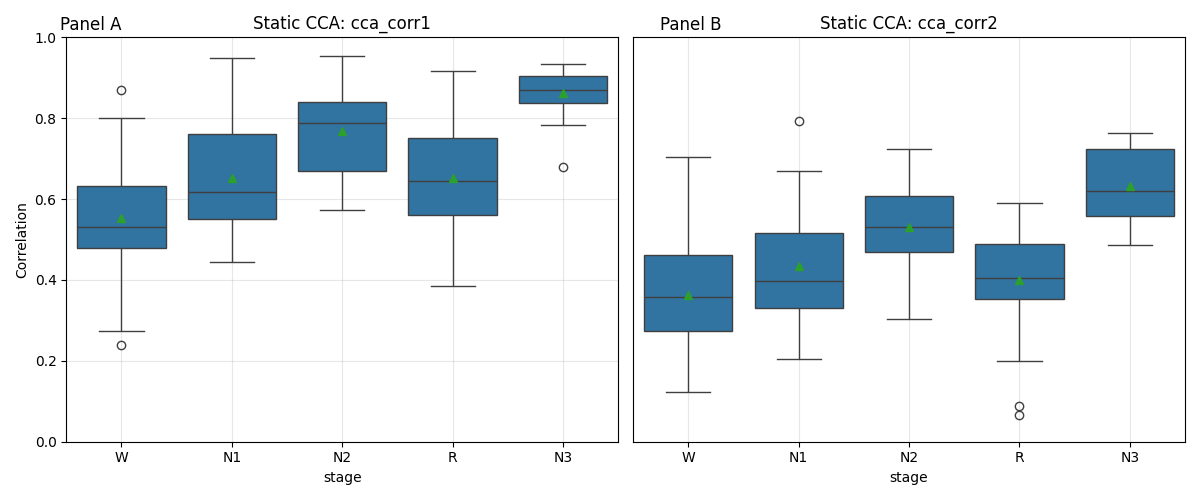
\includegraphics[width=0.8\textwidth]{figure1_static_cca_boxplots.png}% % static_cca_analysis/cca_corr_by_stage.png
\caption{Static EEG--EOG coupling by sleep stage. Boxplots summarize the first (Panel A, $\rho_1$) and second (Panel B, $\rho_2$) canonical correlations from CCA computed on stage-wise concatenated data ($N=29$ participants; stages W, N1, N2, N3, R). Both $\rho_1$ and $\rho_2$ increase with sleep depth (W $\rightarrow$ N3), whereas REM is comparable to N2 on average but more variable. Boxes show interquartile range (IQR) with median; whiskers indicate 1.5$\times$IQR.}\label{fig:figure1}
\end{figure}%

\subsection{Time-Resolved CCA Analysis}

Sliding windows (30 s, $50\%$ overlap) reproduced the pattern with finer resolution. Aggregated $\rho_1$ ranged from 0.73 $\pm$ 0.13 (Wake) to 0.87 ± 0.07 (N3); $\rho_2$ from 0.45 $\pm$ 0.17 to 0.65 $\pm$ 0.11 (Fig.~\ref{fig:figure2}). Variability diminished with depth, and 10-min bins revealed stable plateaus in N2/N3 but fluctuating profiles in REM and Wake. Transition phases (e.g., N1) showed inconsistent coupling patterns.
Local stationarity analysis confirmed that the majority of 30-second windows met standard weak stationarity criteria. Specifically, 85\% of the time-resolved segments passed the ADF test and 61\% passed the KPSS test, with both tests agreeing on stationarity in 56\% of cases. Only 10.5\% of windows were classified as non-stationary by both tests. These results justify the use of fixed-length sliding windows for estimating coupling dynamics.%
\begin{figure}[!t]
\centering
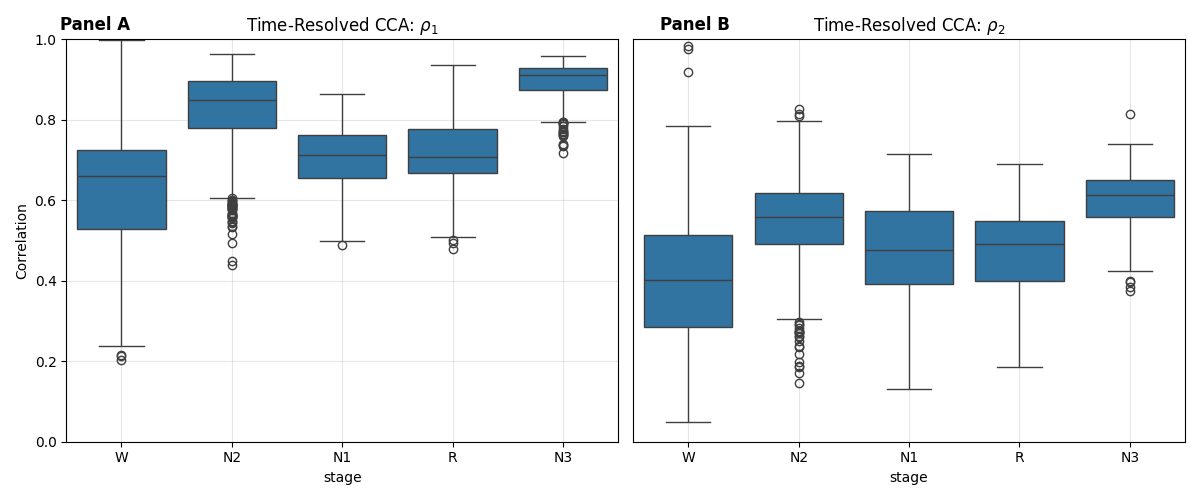
\includegraphics[width=0.8\textwidth]{figure2_time_resolved_boxplots.png}% % static_cca_analysis/cca_corr_by_stage.png
\caption{Time-resolved coupling distributions by stage. Using 30~s windows (15~s step) across the night, boxplots show the distributions of $\rho_1$ (Panel A) and $\rho_2$ (Panel B) within each stage. The same stage ordering appears as in the static analysis, with tighter, higher correlations in N2/N3 and broader, lower correlations in Wake and REM.}\label{fig:figure2}
\end{figure}%
\vspace{0pt}%

\subsection{Distributional Complexity of Coupling Dynamics}
\vspace{0pt}%
Entropy was highest in Wake and REM and lowest in N3 (Fig.~\ref{fig:figure3}). Skewness (between -0.5 and 0.5) remained near zero, but kurtosis was elevated in Wake/REM, suggesting occasional extreme coupling events.%
\begin{figure}[!t]
\centering
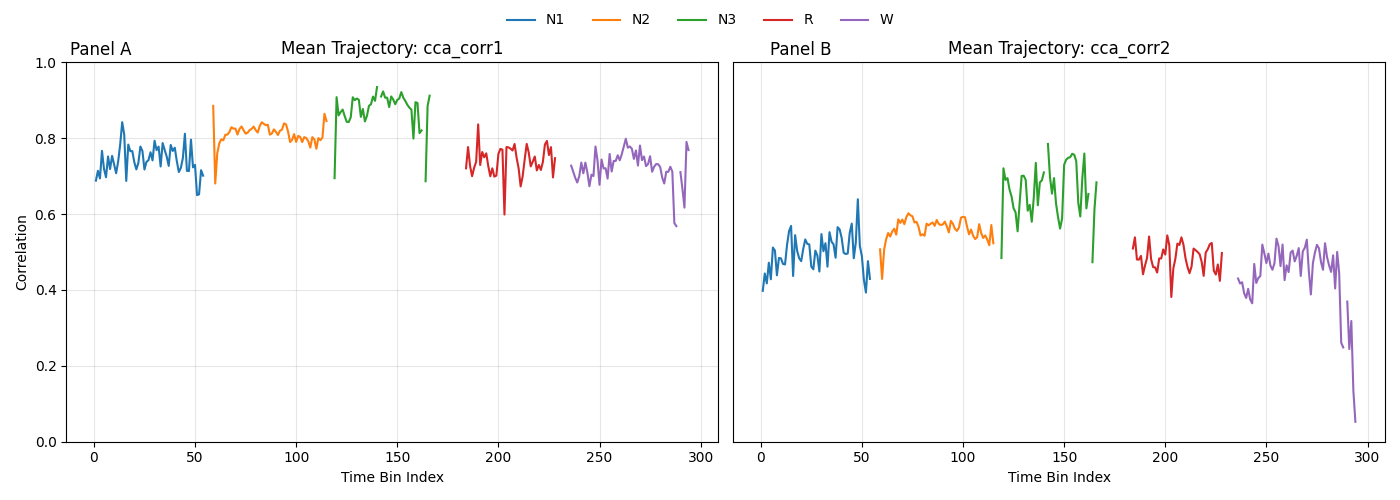
\includegraphics[width=0.8\textwidth]{figure3_cca_trajectories.png}% % static_cca_analysis/cca_corr_by_stage.png
\caption{Mean coupling trajectories by stage. Stage-specific trajectories of the first (Panel A, $\rho_1$) and second (Panel B, $\rho_2$) canonical correlations averaged across subjects over time-bin indices (10~min bins). N2/N3 exhibit relatively flat, stable coupling plateaus, while Wake and REM show more pronounced temporal variability.}\label{fig:figure3}
\end{figure}%
\vspace{0pt}%

\subsection{Projection Statistics and Downsampled Components}
\vspace{0pt}%
Mean and variance of the individual canonical projections showed no stage effect (all ANOVA p>0.17; Fig.~\ref{fig:figure4}). Thus, stage differences stem from correlation structure rather than projection amplitude.
We also evaluated how much signal variance was captured by each canonical variate. On average, the first component explained 52-57\% of EEG variance and 52-63\% of EOG variance across sleep stages. In deeper stages such as N3, variance was more evenly distributed across components, while in REM and Wake, the first component dominated. These findings indicate a low-dimensional, structured coupling that varies with brain state.%
\begin{figure}[!t]
\centering
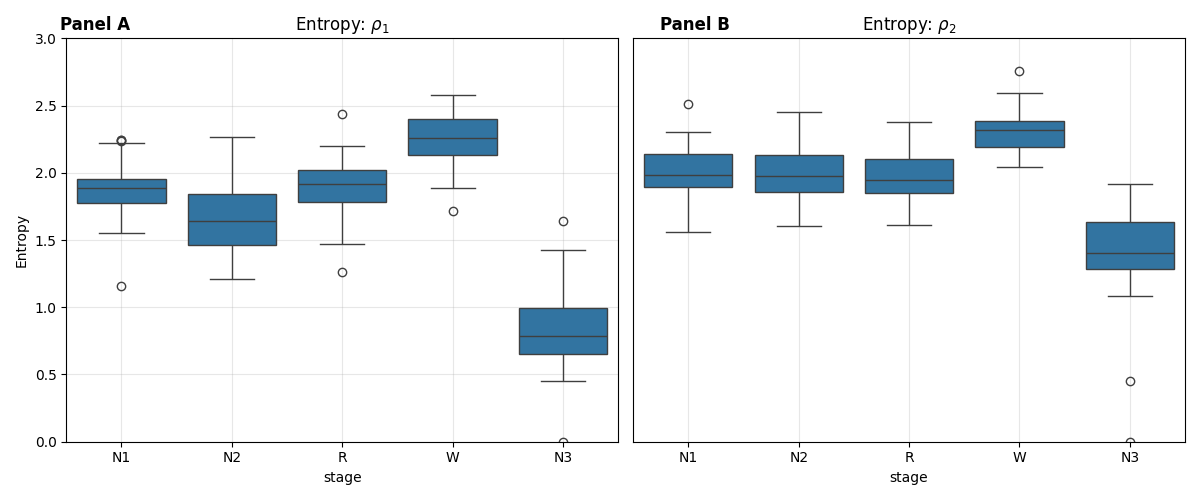
\includegraphics[width=0.8\textwidth]{figure4_entropy_boxplots.png}%
\caption{Within-stage dispersion (entropy) of time-resolved coupling. Subject-level Shannon entropy of $\rho_1$ (Panel A) and $\rho_2$ (Panel B) distributions computed within each stage. Entropy is lowest in N3 and highest in Wake and REM, indicating narrower and broader coupling distributions, respectively. One value per subject and stage.}\label{fig:figure4}
\end{figure}%
\vspace{0pt}%

\section{Discussion}
This study quantified the strength and dynamics of the shared EEG--EOG subspace across human sleep, using canonical correlation analysis (CCA) at two complementary scales: (i) a static, stage-wise summary and (ii) a time-resolved view with short sliding windows. Across both approaches, coupling increased with sleep depth and was most stable in N2/N3, whereas Wake and REM exhibited broader, more fluctuating distributions. Taken together, these patterns suggest that as cortical and oculomotor systems enter deeper non-REM sleep, their shared low-dimensional activity becomes more coherent and less variable.

\textbf{Physiological interpretation.}
Higher and more stable coupling in N2/N3 is consistent with reduced oculomotor activity, stronger large-scale cortical synchronization, and a relative quiescence of rapid eye movements. Conversely, greater spread in Wake and REM likely reflects mixtures of ocular events (e.g., saccades, blinks or REMs)~\cite{hobson2010, mccarley1994}, arousal fluctuations, and heterogeneous cortical states. In N1, modest but consistent coupling may reflect coordinated slow eye movements and low-frequency EEG patterns (waning alpha/theta), which aligns with known challenges in detecting N1 from EEG alone~\cite{xu2025}. We observed that in most stages, a single dominant canonical dimension ($\rho_1$) is accompanied by a smaller second dimension ($\rho_2$). This pattern suggests that most of the shared variance lies in a low-dimensional subspace, with smaller residual structure that differs by stage.

\textbf{Temporal dynamics and dispersion.}
Time-resolved trajectories showed that N2/N3 maintain elevated coupling with limited drift, while Wake and REM oscillate more strongly. The entropy analysis formalized this observation: coupling distributions were narrowest in N3 and broadest in Wake/REM. Entropy here complements correlation magnitudes by describing how \emph{concentrated} or \emph{diffuse} the coupling is within a stage, capturing variability beyond central tendency.

\textbf{Methodological contributions.}
Two checks strengthen the interpretation of our estimates. First, the explained-variance profiling of canonical variates confirmed that the leading modes capture a substantive fraction of the shared structure, supporting the use of a low-dimensional shared space. Second, our assessment of within-stage stationarity (local behavior across windows) supports the validity of pooling windows within stages for summary statistics. Together, these steps help distinguish robust, stage-specific coupling from artifacts of windowing or overfitting.

\textbf{Implications.}
Coupling strength and dispersion jointly characterize stage-specific brain--eye coordination: deeper non-REM sleep is marked by stronger, more orderly shared activity, while Wake/REM express broader, more volatile coupling. Such signatures may be informative for automatic sleep staging, for tracking micro-arousal dynamics, or for probing disorders that alter ocular or cortical control (e.g., REM behavior disorder, insomnia, or sedative effects). Because CCA is transparent and low-dimensional, these metrics can be integrated with standard PSG pipelines and interpreted alongside known physiology.

\textbf{Limitations.}
Our sample size is modest; not all participants express all stages with equal duration, which can bias distributional estimates. We restricted EEG to a small set of central/occipital derivations and used bipolar EOG channels; different montages, references, or artifact pipelines could shift absolute values. CCA is linear and agnostic to directionality, so nonlinear or directed interactions may be underrepresented. Window length and step (30~s/15~s) were chosen for interpretability and alignment with sleep scoring; alternative scales could reveal finer microstructure. Finally, coupling can reflect both genuine shared neural sources and volume-conducted or reference-related contributions; future work combining source modeling or cross-modal control analyses will help disambiguate these factors.
\FloatBarrier
\textbf{Conclusion.}
Using canonical correlation analysis, we showed that EEG and EOG share a compact, stage-dependent subspace whose strength increases and whose dispersion narrows with sleep depth. Static summaries and time-resolved windows converged on the same picture: N2/N3 exhibit stronger, more stable coupling, while Wake and REM are weaker and more variable. Entropy provided an orthogonal descriptor of within-stage dispersion that complements correlation magnitudes. These simple, interpretable metrics can be embedded in routine PSG analysis and may aid studies of sleep microstructure and pathology. Future work should expand channel coverage, test nonlinear and directional measures, and evaluate clinical sensitivity across disorders and interventions.

\subsection*{Project's repository}
The code and analysis for this project is available at \url{https://github.com/Eager1Beaver/bespace}.

\renewcommand{\baselinestretch}{1.5}
%\singlespacing
%\renewcommand\bibname{Bibliography}
\bibliographystyle{abbrv} %abbrv
\phantomsection     % 
%\cleardoublepage    % 
\bibliography{report}

\end{document}
